\subsection{Approximationserhaltende Reduktionen (AP-Reduktionen)}
\label{sec:ap-reduktionen}

\paragraph{Idee}
Gegeben ein Problem $U_1$ das bekanntermassen kein PTAS zulässt.
Zeige dass ein anderes Problem $U_2$ auch kein PTAS zulässt durch Reduktion von $U_1$ auf $U_2$.
Wichtig: die Reduktion muss die Approximationsgüte erhalten.

\paragraph{AP-reduzierbar}
Seien $U_1 = (L_1, M_1, cost_1, goal_1)$ und $U_2$ Optimierungsprobleme.
$U_1$ ist \emph{AP-reduzierbar} auf $U_2$, notiert $U_1 \leq_{AP} U_2$, falls Funktionen
\begin{itemize}
    \item $ F \cl L_1 \times \Q^+ \mapsto L_2 $
    \item $ H \cl L_1 \times \Q^+ \times \bigcup_{y \in L_2} M_2(y) \mapsto \bigcup_{x \in L_1} M_1(x) \quad ; \; x \geq 0 $
\end{itemize}
und eine Konstante $\alpha > 0$ existieren so dass:
\begin{enumerate}[label=(\roman*)]
    \item $\forall x \in L_1$ mit $M_1(x) \neq \emptyset$, $\forall \varepsilon \in \Q^+$ : \quad
        $F(x, \varepsilon) \in L_2$ und $M_2(F(x, \varepsilon)) \neq \emptyset$
    \item $\forall x \in L_1$ mit $M_1(x) \neq \emptyset$, $\forall \varepsilon \in \Q^+$,
        $\forall y \in M_2(F(x, \varepsilon))$ : \quad
        $H(x, \varepsilon, y) \in M_1(x)$
    \item $F, H$ in Zeit poly$(|x|, |y|)$ berechenbar für ein fixes $\varepsilon$
    \item Zeitkomplexität von $F,H$ wächst nicht mit $\varepsilon$ für alle fixen $|x|, |y|$
        \footnote{Nicht notwendig, aber wünschenswert.}
    \item $\forall x \in L_1$, $\forall \varepsilon \in \Q^+$, $\forall y \in M_2(F(x, \varepsilon))$ : \quad
        $$ R_{U_2}(y, F(x,\varepsilon)) \leq 1 + \frac{\varepsilon}{\alpha}
        \; \implies \; R_{U_1}(H(x, \varepsilon, y), x) \leq 1 + \varepsilon $$
        D.h. die Approximationsgüte bleibt erhalten ($\alpha$ erlaubt eine leichte Veränderung).
\end{enumerate}

\begin{figure}[h]
    \centering
    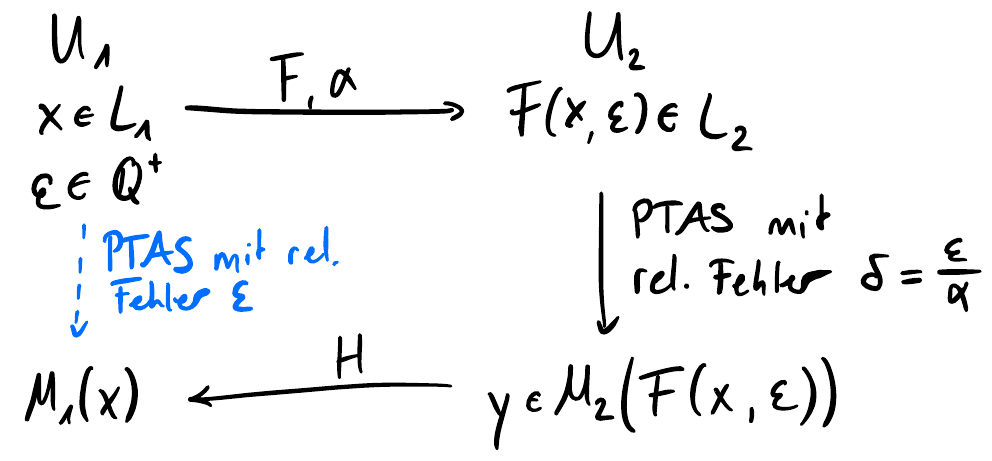
\includegraphics[width=0.4\textwidth]{images/ap-reduktionen.png}
    \caption{AP-Reduktionen}
\end{figure}

\paragraph{Lemma}
Seien $U_1, U_2$ Optimierungsprobleme wie oben.
Falls $U_1 \leq_{AP} U_2$, so gilt:
$$ \exists \text{ PTAS für } U_2 \implies \exists \text{ PTAS für } U_1 $$
$$ \not \exists \text{ PTAS für } U_1 \implies \not \exists \text{ PTAS für } U_2 $$

\underline{Beweis}: offensichtlich. Siehe Buch S.320.

\paragraph{APX-vollständig}
Ein Problem $U \in NPO$ heisst \emph{APX-vollständig (APX-complete)} falls gilt:
\begin{enumerate}
    \item $U \in APX$
    \item $\forall W \in APX \cl W \leq_{AP} U$
\end{enumerate}

\paragraph{Max-SAT}
Eingabe: Formel $C = C_1 \wedge ... \wedge C_m$ in KNF über Variablen $x_1, ..., x_n$.
Ziel: Belegung die die Anzahl erfüllter Klauseln maximiert.

\paragraph{Max-CLIQUE (Max-CL)}
Eingabe: ungerichteter Graph $G$.
Ziel: Clique in $G$ mit maximaler Knotenanzahl.

\paragraph{Lemma}
Max-SAT $\leq_{AP}$ Max-CLIQUE

\underline{Beweis:} Konstruktion (sei $C_i = l_{i1} \vee ... \vee l_{ij_i}$):
\begin{itemize}
    \item $\alpha = 1$
    \item $ F(C, \varepsilon) = F(C) = G_C = (V,E) $ mit
        $ V = \{ (i, k) \st 1 \leq i \leq m \; , \; 1 \leq k \leq j_i \}$
        (jede occurence eines Literals hat einen Knoten) und
        $ E = \{ \{ (r,s) , (p,q) \} \st r \neq p \; , \; l_{rs} \not \equiv \overline{l}_{pq} \} $
        (keine Kanten innerhalb einer Klausel, und keine Widersprüche)
        \footnote{D.h. $F$ ist unabhängig von $\varepsilon$.}
    \item $ H $ wählt eine Belegung $\gamma$ wie folgt:
        für die Literale in der gefundenen Max-Clique, wähle $x_i=1$ und $\overline{x}_i=0$.
        Wähle alle anderen Literale beliebig.
\end{itemize}
Dies erfüllt unsere Bedingungen:
(i) Eingabe wird gemapped. (ii) Ausgabe wird gemapped.
(iii) $F, H$ in Polynomzeit berechenbar. (iv) $F, H$ unabhängig von $\varepsilon$.
(v) Jede Clique $Q$ der Grösse $q$ erfüllt $\geq q$ Klauseln.
Jede Belegung die $r$ Klauseln erfüllt, bestimmt eine Clique der Grösse genau $r$.
\\
$\implies cost_{Max-SAT}(H(G_C)) \geq cost_{Max-CLIQUE}(Q)$.

\begin{figure}[h]
    \centering
    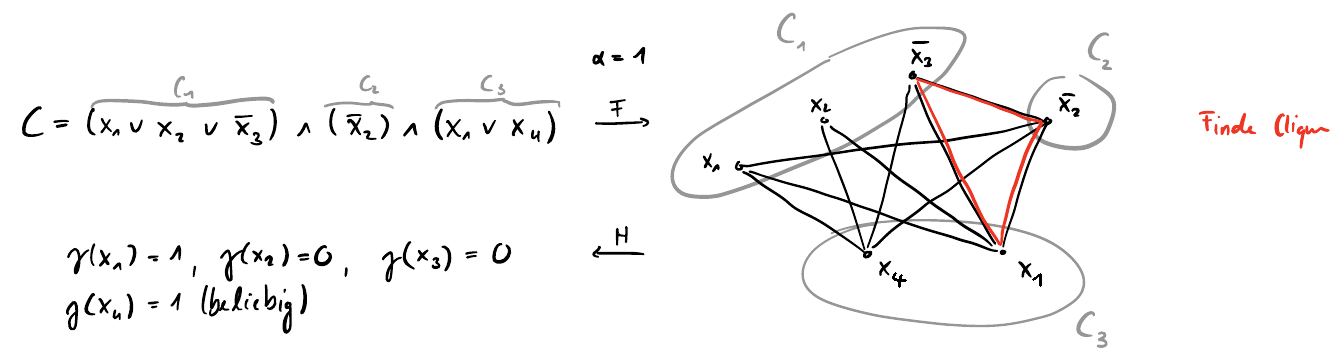
\includegraphics[width=0.8\textwidth]{images/ap-reduktion-beispiel.png}
    \caption{Beispiel AP-Reduktion Max-SAT $\leq_{AP}$ Max-CLIQUE}
\end{figure}

\paragraph{Fazit}
AP-Reduktionen sind intuitiv, aber in der Praxis schwer zu finden.
